\section{Robustness, ablations and failure analysis}
\subsection{Missing ratings and corrupted observations}
\begin{table}[!htbp]\centering\footnotesize
\begin{tabular}{@{}lrrrr@{}}\toprule
Condition & ADF & EP5 & MF-MAP & GMRF-MAP\\\midrule
main & 0.8980 $\pm$ 0.0049 & 0.8633 $\pm$ 0.0040 & 0.8507 $\pm$ 0.0028 & 0.8501 $\pm$ 0.0031\\
retain\_0.25 & 0.9217 $\pm$ 0.0041 & 0.9199 $\pm$ 0.0051 & 0.9178 $\pm$ 0.0042 & 0.9100 $\pm$ 0.0038\\
retain\_0.5 & 0.9102 $\pm$ 0.0039 & 0.8920 $\pm$ 0.0049 & 0.8810 $\pm$ 0.0039 & 0.8775 $\pm$ 0.0041\\
noise\_0.1 & 0.9129 $\pm$ 0.0036 & 0.8910 $\pm$ 0.0036 & 0.8827 $\pm$ 0.0029 & 0.8797 $\pm$ 0.0030\\
noise\_0.2 & 0.9386 $\pm$ 0.0030 & 0.9326 $\pm$ 0.0022 & 0.9317 $\pm$ 0.0023 & 0.9248 $\pm$ 0.0018\\
cold\_items & 1.0703 $\pm$ 0.0079 & 1.0781 $\pm$ 0.0068 & 1.0622 $\pm$ 0.0060 & 1.0545 $\pm$ 0.0077\\
cold\_users & 0.9837 $\pm$ 0.0137 & 0.9861 $\pm$ 0.0146 & 0.9935 $\pm$ 0.0115 & 0.9916 $\pm$ 0.0117\\
\bottomrule\end{tabular}

\caption{Expected-rating test RMSE, mean $\pm$ sample SD over seeds 42--44.
The clean row uses these same three seeds. Cold-start rows evaluate different
restricted test populations and should not be ranked directly against the clean row.}
\end{table}

Reducing training availability increases error for all methods. At 25\%
retention, the graph reduces MF-MAP RMSE from 0.9178 to 0.9100; at 50\%,
from 0.8810 to 0.8775. The corresponding gains, 0.0077 and 0.0036, are larger
than the clean three-seed gain of 0.0006. Sharing evidence is more useful when
each movie has less direct support. This supports the variance-reduction
hypothesis under random removal, while not establishing robustness to actual
nonrandom exposure or missing-not-at-random ratings.

With 10\% corrupted labels, MF-MAP and GMRF-MAP have RMSE 0.8827 and 0.8797;
at 20\%, 0.9317 and 0.9248. The graph mitigates some degradation but does not
recover clean-data performance. Both the training target and the residual
similarities are affected by corruption. The graph helps here despite that
imperfect evidence, consistent with useful smoothing; this experiment does
not identify a universally optimal graph or realistic user-error mechanism.

EP5 remains better than ADF in aggregate, but its advantage becomes small
under sparse or heavily corrupted training. At 25\% retention, seed 43's EP5
is slightly worse than ADF. Repeated inference cannot create reliable evidence
that is absent and may reinforce misspecified observations. These stress
comparisons are descriptive three-seed results, not independent-dataset
significance tests.

\begin{figure}[!htbp]\centering
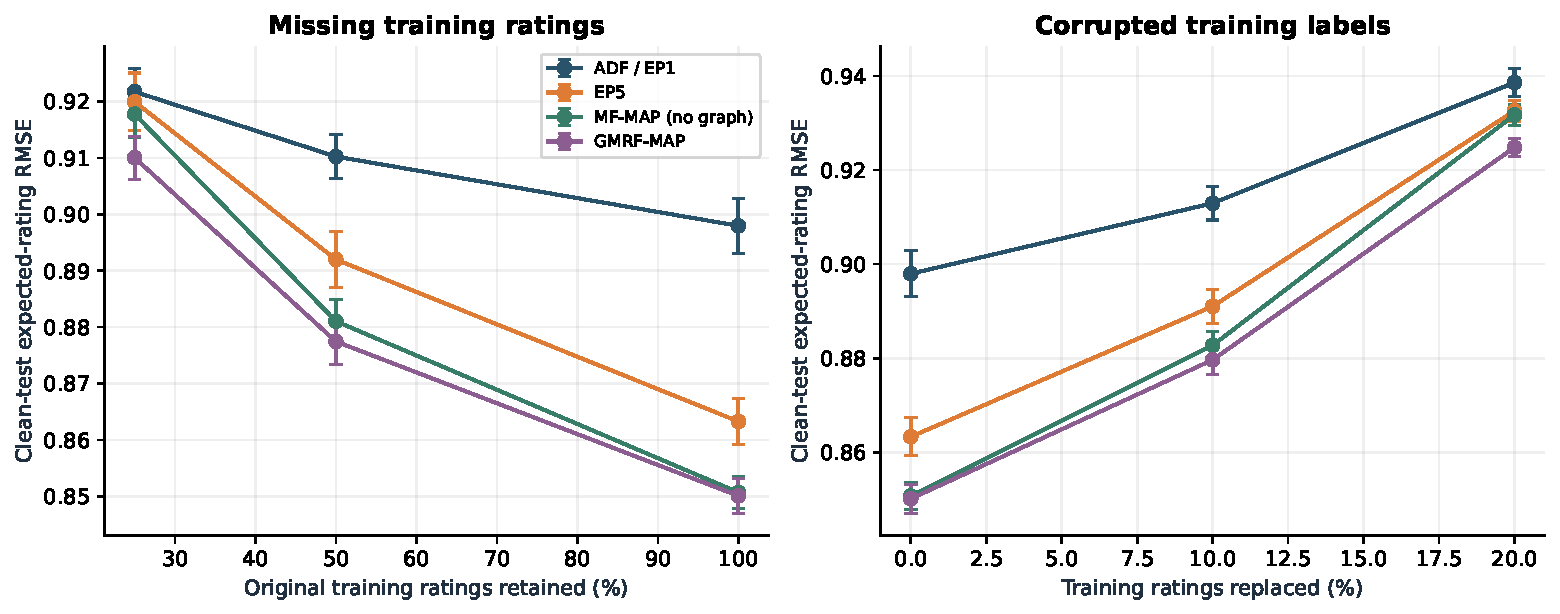
\includegraphics[width=\linewidth]{../../Results/analysis/plots/robustness.pdf}
\caption{Missing-data and label-noise sensitivity. All evaluations use clean
test labels; error bars show sample SD across the same three seeds.}
\end{figure}

\subsection{Which graph components matter?}
\begin{table}[!htbp]\centering\small
\begin{tabular}{@{}lrr@{}}\toprule
Graph condition & MF-MAP RMSE & GMRF-MAP RMSE\\\midrule
main & 0.8507 $\pm$ 0.0028 & 0.8501 $\pm$ 0.0031\\
ratings\_only & 0.8507 $\pm$ 0.0028 & 0.8499 $\pm$ 0.0031\\
genres\_only & 0.8507 $\pm$ 0.0028 & 0.8510 $\pm$ 0.0031\\
graph\_top\_5 & 0.8507 $\pm$ 0.0028 & 0.8497 $\pm$ 0.0031\\
graph\_top\_50 & 0.8507 $\pm$ 0.0028 & 0.8505 $\pm$ 0.0031\\
\bottomrule\end{tabular}

\caption{Graph ablations at fixed $\gamma=10$, three seeds. The graph-free
baseline is unchanged across clean graph variants.}
\end{table}
Ratings-only edges give mean RMSE 0.8499, mixed edges 0.8501, and genre-only
edges 0.8510, versus 0.8507 without a graph. Thus coarse genres alone do not
improve this warm-interaction benchmark. They can connect movies whose
audiences or rating patterns differ; adding metadata is not automatically
beneficial. Genre information still supplies connections for unseen items,
which is a different evaluation setting.

Top-5 neighbours give RMSE 0.8497, whereas top-50 gives 0.8505. More edges do
not necessarily carry more useful information. Combined with the poorer
validation result at strength 100, this reveals an oversmoothing risk.
These topology variants are exploratory diagnostics. The main configuration
remains top-20, fixed before these test comparisons; we do not select a new
reported winner using their test scores.

\subsection{Controlled cold-start and remaining errors}
For withheld movies, GMRF-MAP improves the matching baseline from 1.0622 to
1.0545 RMSE. Genre connections can transfer neighbouring traits when a movie
has no training observations, but its own rating bias cannot be estimated.
Error remains much higher than on the warm main benchmark. EP5 is worse than
ADF here (1.0781 versus 1.0703), another counterexample to universal EP
superiority.

For withheld users, ADF has RMSE 0.9837, EP5 0.9861, MF-MAP 0.9935 and
GMRF-MAP 0.9916. The movie graph offers no user metadata or user-specific
evidence, so it cannot personalize a completely unseen user. It slightly helps
its matching MAP baseline but does not beat ADF in this setting. This limits
the claim that a movie network resolves cold-start in general.

\begin{figure}[!htbp]\centering
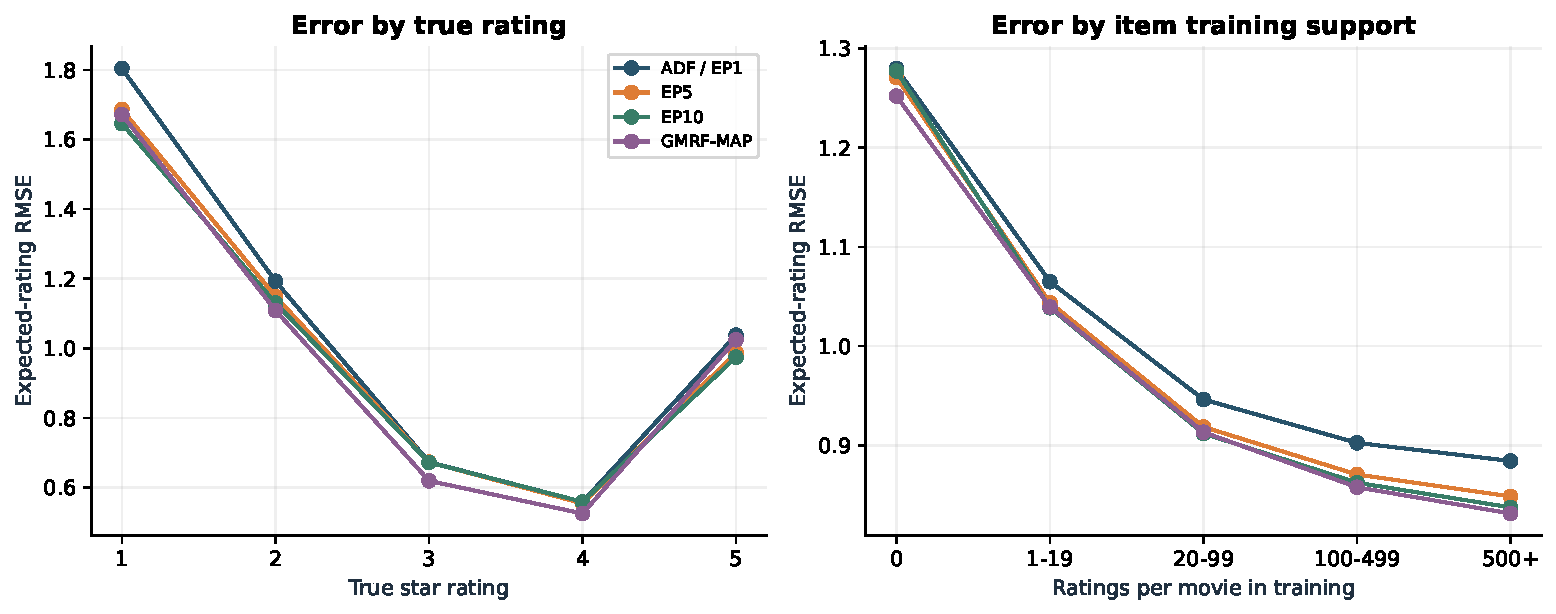
\includegraphics[width=\linewidth]{../../Results/analysis/plots/error_analysis.pdf}
\caption{Descriptive pooled errors by true rating and movie support. Pooled
split observations overlap; the curves do not represent independent samples.}
\end{figure}

The main benchmark's five-star error is 1.0245 for GMRF-MAP versus 0.9748 for
EP10, despite GMRF's better aggregate RMSE. Its advantages are stronger around
three/four-star observations. The expected-rating decision and regularization
shrink predictions toward the centre, overpredicting low ratings and
underpredicting high ratings. An overall score therefore hides meaningful
class-specific failures.

Low-support movies are harder for every method. The natural zero-training-item
bin contains only 83 pooled test observations across five overlapping splits;
its curve should not support a broad cold-start claim. The controlled
withheld-item experiment is the more appropriate evidence. Support strata
also differ in movie composition, so their error differences are descriptive,
not causal estimates of adding ratings.

\subsection{Prior, damping and order sensitivity}
\begin{table}[!htbp]\centering\small
\begin{tabular}{@{}lrr@{}}\toprule
EP5 variant & RMSE & NLL\\\midrule
ADF\_reshuffled & 0.8984 $\pm$ 0.0049 & 1.2526 $\pm$ 0.0046\\
damping\_0.25 & 0.8752 $\pm$ 0.0048 & 1.2292 $\pm$ 0.0041\\
damping\_1 & 0.8529 $\pm$ 0.0038 & 1.2078 $\pm$ 0.0027\\
prior\_0.1 & 0.8672 $\pm$ 0.0043 & 1.2216 $\pm$ 0.0036\\
prior\_0.5 & 0.8650 $\pm$ 0.0039 & 1.2195 $\pm$ 0.0031\\
reshuffled & 0.8638 $\pm$ 0.0039 & 1.2183 $\pm$ 0.0030\\
\bottomrule\end{tabular}

\caption{Fixed EP5 sensitivity variants, mean $\pm$ SD over seeds 42--44.
Each varies one operating choice; the main configuration is not reselected
using these test outcomes. Reshuffled ADF is the first pass of that order.}
\end{table}
Prior strength changes regularization, damping changes the size of cached-site
replacements, and reshuffling changes the sequence of approximate updates.
These comparisons expose dependence on operating choices rather than proving
that the original settings are optimal. Their validation trajectories and
test metrics are supplied together. A broader validation-only search would
be needed to compare optimized method families fairly; this finite study
does not claim exhaustive tuning or order invariance.

With undamped replacement after the first pass (outer damping 1), EP5 reaches
mean RMSE 0.8529 across the three sensitivity seeds, compared with 0.8633 for
the original EP5 setting and 0.8501 for GMRF-MAP on those same seeds.
Thus tuning the inference schedule closes much of the apparent gap. This is
an exploratory fixed-variant comparison, not a validation-selected replacement
for the five-seed main method. It further limits any claim that graph structure
alone explains superior performance.
